% !TEX root = morphkasten.tex

\section{Kamera}


%##############
\subsection{Raspberry Pi Cam}

\begin{figure}[h!]%Position festigen
\centering
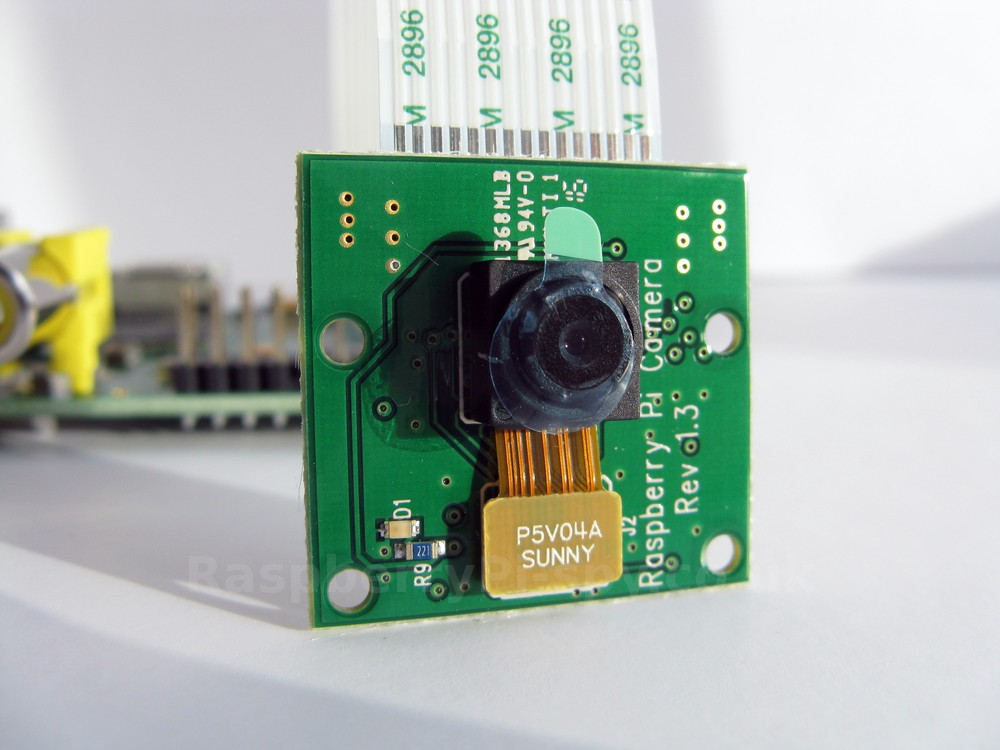
\includegraphics[width=0.5\textwidth]{fig/raspberry-pi-camera-module.jpg}
\caption{Pi Cam (Quelle: https://www.raspberrypi.org)}
\label{fig:PiCam}
\end{figure}

\begin{table}[h]
\begin{tabular}{p{0.5\textwidth} | p{0.5\textwidth}}


 \textbf{Vorteile} & \textbf{Nachteile} \\ \hline
	 
\begin{itemize}
\item Tiefe Anschaffungskosten
\item Kleine Baugrösse
\item Grosse Community
\item OpenSource Treiber
\item Gute Auflösung
\end{itemize}

 
 &
 
\begin{itemize}
\item Fester Fokus auf 1m
\item Relativ geringer Winkel mit 53.5°
\item Halterung muss erstellt werden
\item MIPI Schnittstelle erforderlich
\end{itemize}

\end{tabular}
\end{table}

\begin{table}[h]
\begin{tabular}{p{0.5\textwidth}p{0.5\textwidth}}


 \textbf{Risiken} & \\ \hline
	 
\begin{itemize}
\item Fahrbahn kann nicht vollständig erfasst werden in der Kurve
\item Objekte können nicht vollständig erfasst werden.
\item Kompatibilität zu Minicomputer eingeschränkt (Nur Rasp Pi und Banana Pi)
\end{itemize}
&
\begin{itemize}
\item Kein Autofokus: Scharfstellung nicht sichergestellt
\item Farbverhalten beu unterschiedlichen Lichtverhältnissen 
\end{itemize}

 
\end{tabular}
\end{table}

\pagebreak


%##############
\subsection{Webcam}
Grafik

\begin{table}[h]
\begin{tabular}{p{0.5\textwidth} | p{0.5\textwidth}}


 \textbf{Vorteile} & \textbf{Nachteile} \\ \hline
	 
\begin{itemize}
\item Vorteil 1
\item Vorteil 2
\item Vorteil 3
\item ...
\end{itemize}

 
 &
 
\begin{itemize}
\item Nachteil 1
\item Nachteil 2
\item Nachteil 3
\item ...
\end{itemize}

\end{tabular}
\end{table}

\begin{table}[h]
\begin{tabular}{p{0.5\textwidth}p{0.5\textwidth}}


 \textbf{Risiken} & \\ \hline
	 
\begin{itemize}
\item Risiko 1
\item Risiko 2
\end{itemize}
&
\begin{itemize}
\item Risiko 3
\item ...
\end{itemize}

 
\end{tabular}
\end{table}

\pagebreak